\chapter{CHỨC NĂNG ĐIỀU KHIỂN CÓ ĐIỀU KIỆN}
\begin{flushleft}
	\fontsize{12pt}{7pt}\selectfont
	\textit{Chương này sẽ trình bày nội dung tích hợp chức năng điều khiển có điều kiện vào công cụ eXe Learning. Mục đầu tiên sẽ nêu các khái niệm điều khiển có điều kiện cùng những hạn chế của eXe và hướng khắc phục. Để tiện cho người đọc có thể hiểu phần hiện thực ở mục thứ ba, mục kế tiếp sẽ trình bày cơ chế hiện thực điều khiển có điều kiện trên SCORM. Cuối cùng là phần hiện thực tính năng ở mục thứ ba.}
\end{flushleft}

\section{Khái niệm về điều khiển có điều kiện trong SCORM}
\subsection{Khái niệm điều khiển có điều kiện (Conditionaly Navigation)}
		

	\begin{center}
	\begin{figure}[htp]
		\begin{center}
			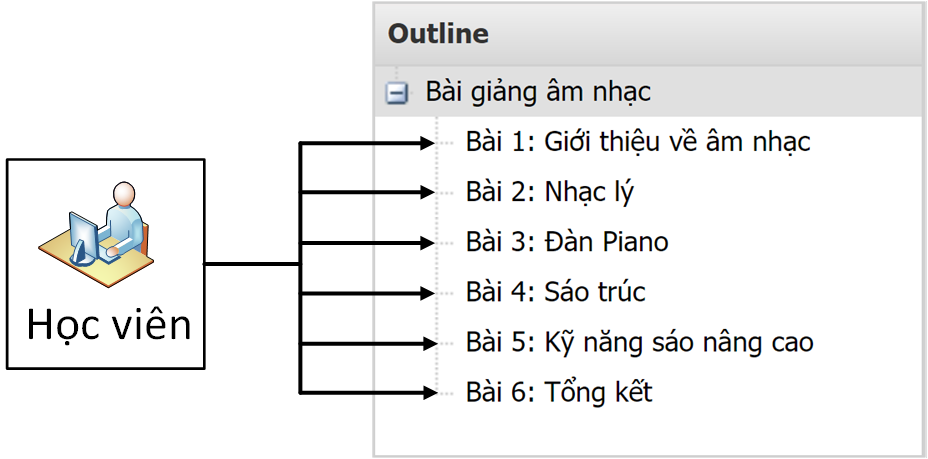
\includegraphics[width=13cm]{Chapter3/Pictures/picture31.png}
		\end{center}
		\caption{Mô hình điều khiển không có điều kiện}
		\label{refpicture12}
	\end{figure}
\end{center}



Hình 3.1 thể hiện ví dụ của một khóa học được soạn thảo bằng eXe hiện tại, khi bắt đầu học, người học có thể ngay lập tức di chuyển vào bất cứ mọi bài trong khóa học. Theo như ví dụ trên thì người học có thể ngay lập tức học \textbf{Bài 6: Tổng kết}, việc này sẽ ảnh hưởng đến thời gian và hiệu suất học tập của người học, vì nếu như chưa trang bị đủ kiến thức của những bài trước mà lại lựa chọn ngay vào học bài tổng hợp ở cuối cùng thì sẽ không đảm bảo việc tiếp thu đầy đủ kiến thức của khóa học. Đây là ví dụ của một mô hình điều khiển không có điều kiện.\\


Chức năng điều khiển có điều kiện sẽ khắc phục được những vấn đề như trên. Chức năng này giúp người soạn thảo có thể thiết lập điều kiện ở mỗi bài, giúp đưa ra một lộ trình học cụ thể. Điều kiện bao gồm tiền điều kiện và hậu điều kiện. Tiền điều kiện là điều kiện mà người học cần thỏa mãn để được vào học một bài học, tiền điều kiện của 1 bài học là bài học mà người học cần phải hoàn thành (thỏa mãn hậu điều kiện) trước khi vào nội dung bài học này. Hậu điều kiện là điều kiện xác nhận người học đã hoàn thành bài học này, hậu điều kiện có thể là thời gian tối thiểu người học phải bỏ ra cho một bài học hoặc phải đạt một số bài kiểm tra nào đó do người biên soạn quy định. Sau đây là ví dụ giúp người đọc dễ hình dung hơn.

\vspace{1cm}

\begin{center}
	\begin{figure}[htp]
		\begin{center}
			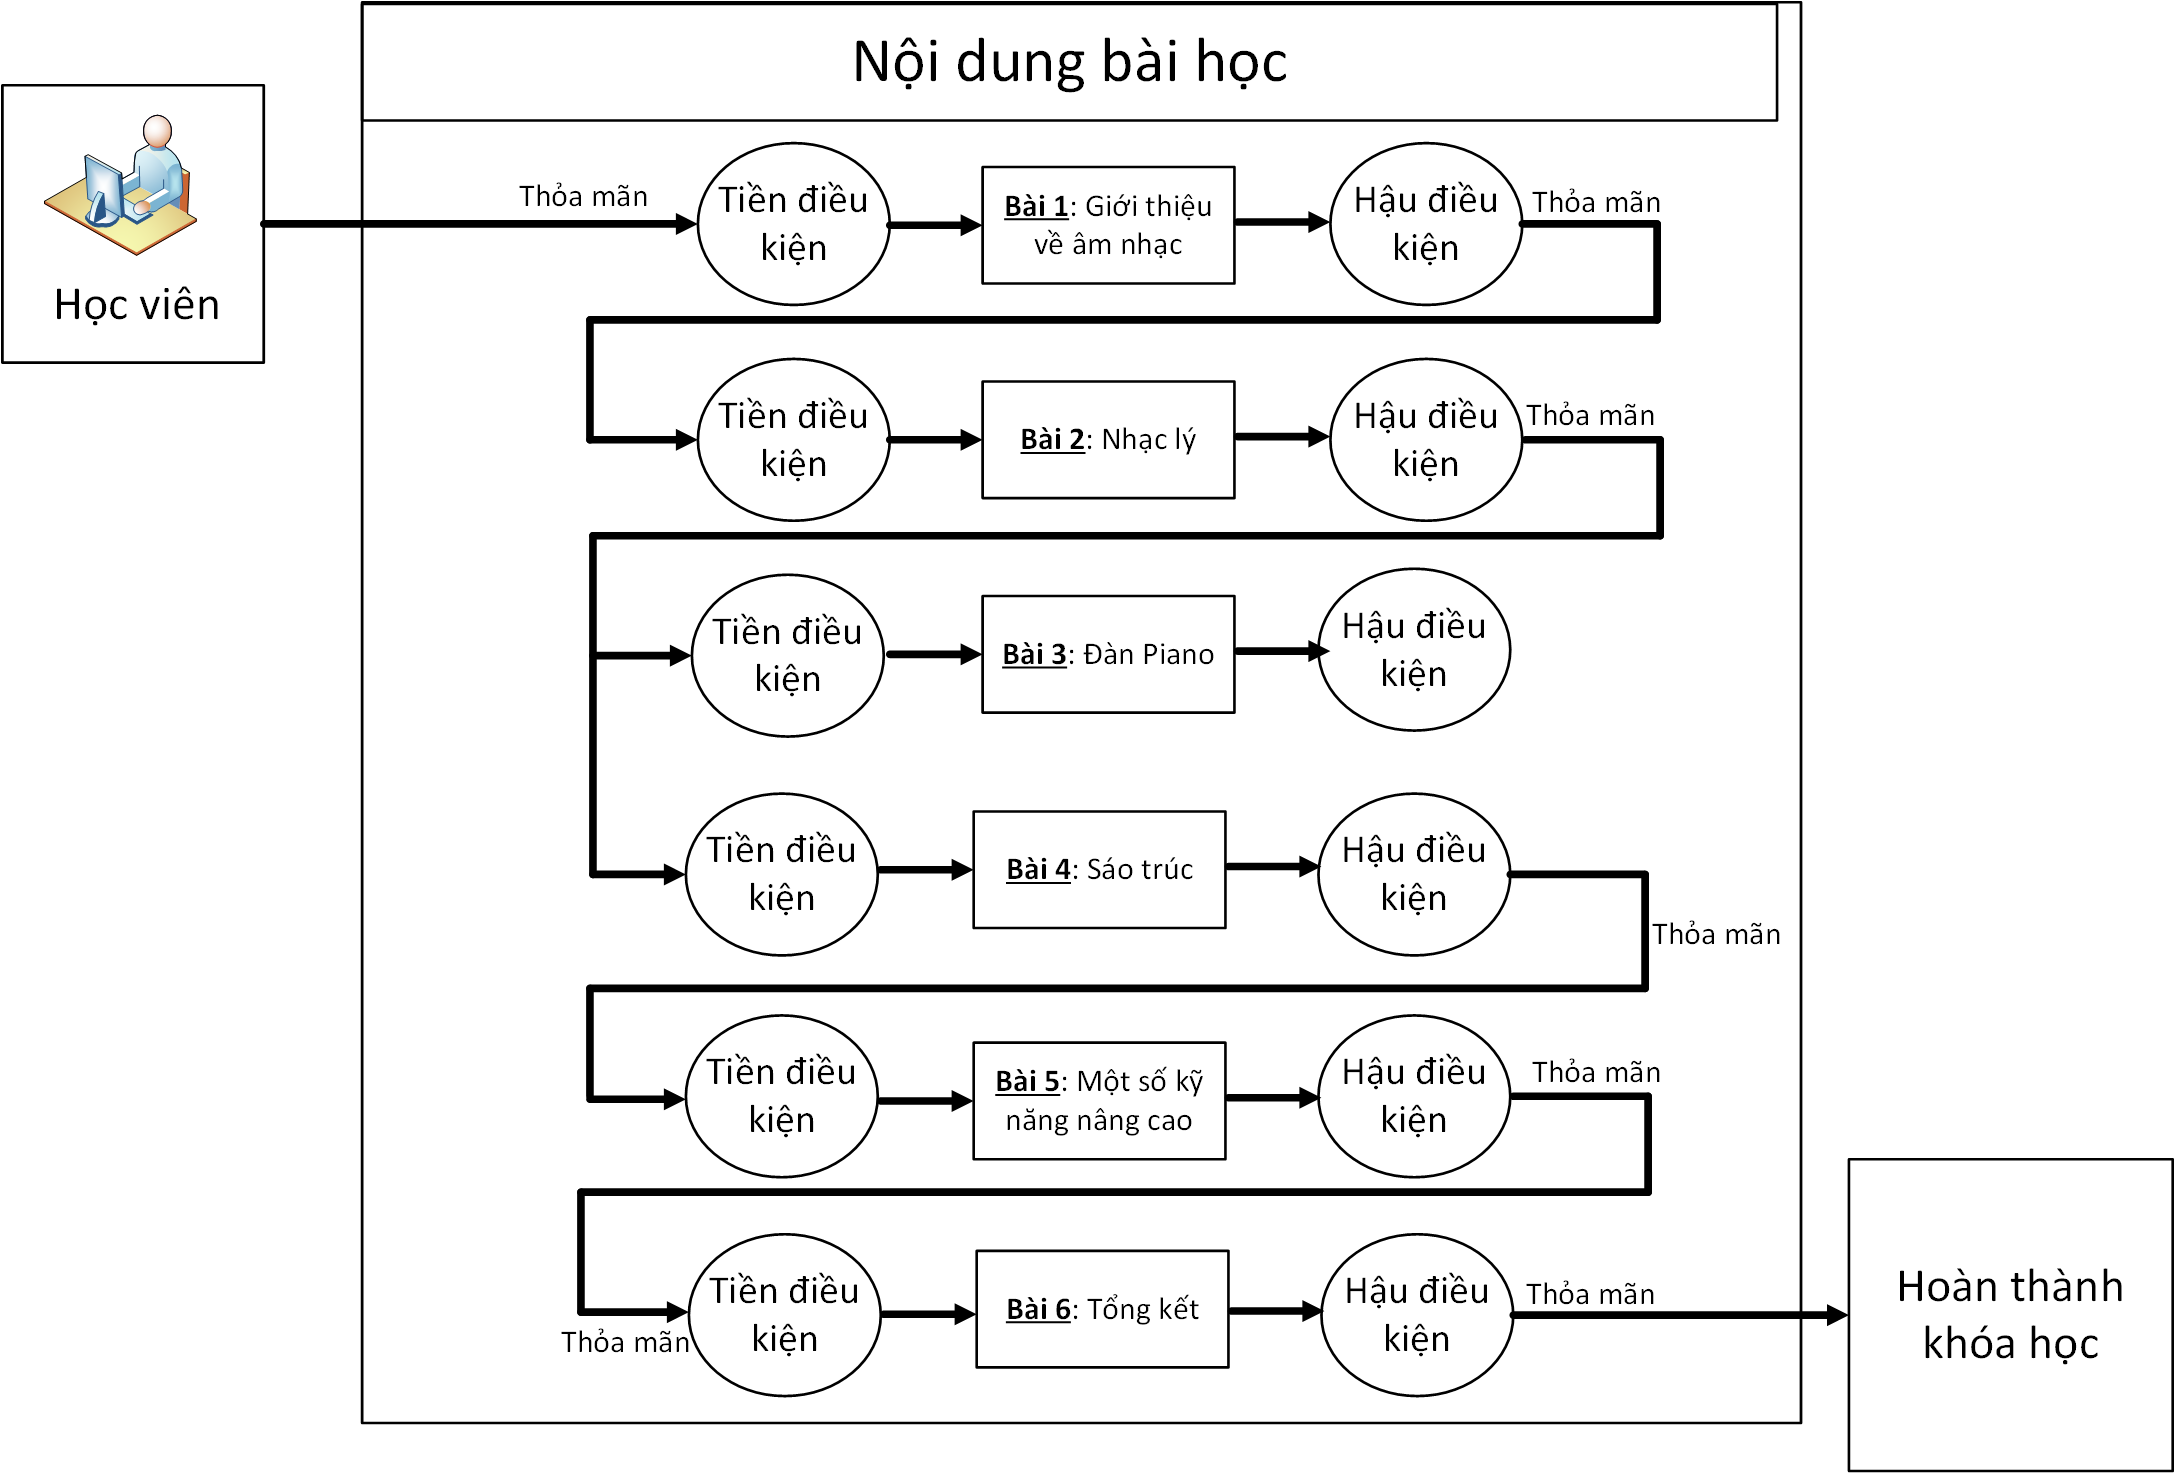
\includegraphics[width=16cm]{Chapter3/Pictures/picture32.png}
		\end{center}
		\caption{Mô hình điều khiển có điều kiện}
		\label{refpicture13}
	\end{figure}
\end{center}


	Hình 3.2 thể hiện ví dụ một mô hình điều khiển có điều kiện. Ở ví dụ này mỗi bài đều được thiết lập tiền điều kiện và hậu điều kiện tương ứng. Đầu tiên học viên sẽ học "Bài 1: Giới thiệu âm nhạc", vì đây là bài đầu tiên của khóa học nên sẽ không cần phải thỏa mãn tiền điều kiện. Tiếp theo học viên muốn học "Bài 2: Nhạc lý" thì học viên cần phải thỏa mãn tiền điều kiện của Bài 2 này, tức hậu điều kiện của Bài 1, hậu điều kiện của Bài 1 có thể là thời gian phải bỏ ra hoặc bài kiểm tra cần đạt tùy theo thiết lập của người soạn thảo. Sau khi hoàn thành Bài 2, học viên có thể lựa chọn tiếp tục học "Bài 3: Đàn Piano" hoặc "Bài 4: Sáo trúc", vì nội dung của 2 bài này độc lập với nhau. Sau khi hoàn thành một trong 2 bài này học viên có thể tiếp tục học "Bài 5: Một số kỹ năng nâng cao" và cuối cùng là "Bài 6: Tổng kết".

\newpage

	Chuẩn SCORM hỗ trợ cho việc xây dựng mô hình điều khiển có điều kiện này bằng cách đưa ra các mô tả dựa vào một tập các thuộc tính, mỗi bài học đều có một tập các thuộc tính này. Mỗi thuộc tính sẽ có hai trạng thái là \textbf{\textit{Enable}} hoặc \textbf{\textit{Disable}} như hình 3.3 mô tả.
	
	\begin{itemize}
		\item \textbf{Enable} là khi các tiền điều kiện của bài này \textbf{\textit{đã được thỏa mãn}} và học viên có thể chọn bài này để học. 
		
		\item \textbf{Disable} là khi các tiền điều kiện của bài học này \textbf{\textit{chưa được thỏa mãn}}, học viên cần phải hoàn thành (thỏa mãn hậu điều kiện) các bài học trước mới có thể vào học bài này. Khi đó bài học này sẽ bị vô hiệu hóa, làm mờ đi và học viên không thể chọn được cho đến khi các tiền điều kiện của nó được thỏa mãn.
	\end{itemize}
	
	

\begin{center}
	\begin{figure}[htp]
		\begin{center}
			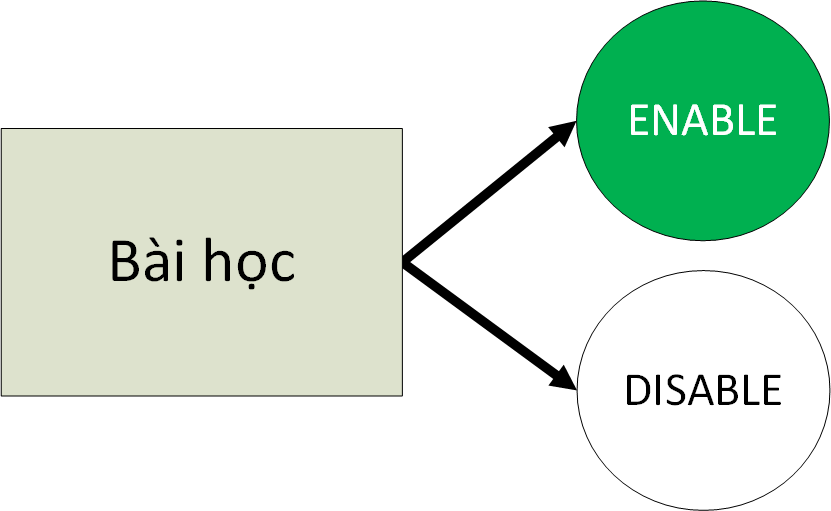
\includegraphics[width=10cm]{Chapter3/Pictures/picture33.png}
		\end{center}
		\caption{Biểu hiện của một bài học đối với người học}
		\label{refpicture42}
	\end{figure}
\end{center}

	
	
\subsection{Mục tiêu đề ra}

	Điều kiện được phát triển để đưa vào mỗi bài học bao gồm hai loại là tiền điều kiện và hậu điều kiện.  Tiền điều kiện là điều kiện mà người học cần thỏa mãn để được vào học một bài học, tiền điều kiện của một bài học là bài học mà người học cần phải hoàn thành (thỏa mãn hậu điều kiện) trước khi vào nội dung bài học này. Hậu điều kiện là điều kiện xác nhận người học đã hoàn thành bài học, hậu điều kiện có thể là thời gian tối thiểu người học phải bỏ ra cho một bài học hoặc phải đạt một số bài kiểm tra nào đó do người biên soạn quy định.\\

	Trong phạm vi Luận Văn này, mục tiêu mà nhóm đặt ra là phát triển các tiền điều kiện và hậu điều kiện nói trên, đồng thời thiết kế giao diện để người soạn thảo đưa các điều kiện này vào bài học và cuối cùng là sinh mã theo chuẩn SCORM có chứa những điều kiện này.

	
\subsection{Các thách thức đặt ra trong quá trình thực hiện}

	Thách thức đầu tiên là sự lỗi thời của các công nghệ được dùng để phát triển eXe. Những công nghệ này đã bị bỏ rơi do cách sử dụng khó khăn, tài liệu hướng dẫn không rõ ràng và phong cách khai báo không tường minh. Bên phía Server, eXe sử dụng hai khung thức của Python là Twisted và Nevow ra đời lần lượt vào năm 2002 và 2004. Còn ở phía Client, eXe sử dụng ExtJS để thiết kế giao diện, ExtJS là một khung thức của Javascript ra đời vào năm 2007. Đây là những công nghệ rất lỗi thời và cộng đồng phát triển của chúng trên Github hầu như không còn. Nevow đã chính thức ngừng phát triển cách đây khoảng năm năm. Tài liệu hướng dẫn của ExtJS rất ít và do đã lâu không cập nhật nên đã bị lỗi thời. \\
	
	Thách thức thứ hai là tài liệu hướng dẫn về những công nghệ này rất hạn chế. Khi tìm kiếm trên google thì số kết quả trả về rất ít, hầu như không có những tài liệu hữu ích và cũng không có những dự án sử dụng những công nghệ này để phát triển. Khi tìm kiếm trên youtube thì hầu như không có Tutorial để tham khảo. Các khóa học về những công nghệ này trên các trang học tập trực tuyến như Udemy, Coursera hay Pluralsight rất ít và cũng không được người học đánh giá cao.\\

	Thách thức thứ ba là cộng đồng phát triển của eXe tương tác rất chậm. Mặc dù diễn đàn của eXe vẫn còn hoạt động nhưng thời gian phản hồi của nó rất chậm do các thành viên phát triển còn rất ít, chỉ có hai người trên diễn đàn này phản hồi với nhóm trong thời gian làm luận văn. Tuy nhiên thời gian nhận được phản hồi cũng rất lâu, khoảng từ hai đến ba tuần cho một vấn đề trong khi thời gian để phát triển luận văn không nhiều.\\
	
	Thách thức thứ tư là hạn chế về thiết kế ban đầu của eXe. Với thiết kế ban đầu của eXe, mỗi bài học chỉ có thể chứa được một SCORM Quiz, hạn chế này đã được các lập trình viên phát triển eXe đưa ra trên diễn đàn theo liên kết \textit{\href{https://exelearning.org/wiki/FAQ}{https://exelearning.org/wiki/FAQ}}. Với thiết kế như vậy, việc người soạn thảo muốn biên soạn nhiều SCORM Quiz trong một bài là không thể. Vì vậy nhóm phải tìm hiểu cách thiết kế ban đầu của iDevice SCORM Quiz trong eXe, sau đó phải tìm cách thay đổi thiết kế này sao cho mỗi bài có thể chứa nhiều SCORM Quiz khác nhau.\\
		


\section{Cơ chế hiện thực chức năng điều khiển có điều kiện}

	SCORM Builder là công cụ hỗ trợ xây dựng dữ liệu theo chuẩn SCORM. SCORM Builder là một công cụ biên soạn (Authoring Tool) cung cấp giao diện soạn thảo bài học, giúp người biên soạn có thể tạo bài giảng, xây dựng nội dung cho bài học và cuối cùng là đóng gói bài học theo chuẩn SCORM. SCORM Builder được sử dụng trong Luận Văn này là eXe.\\
	
	SCORM Engine là công cụ hiển thị nội dung được đóng gói theo chuẩn SCORM. SCORM Engine có thể hiển thị những nội dung mà người soạn thảo đã xây dựng cho bài học, đồng thời tạo ra môi trường giúp nhiều người học có thể tham gia vào bài học này. SCORM Engine được sử dụng trong Luận Văn này là SCORM Cloud.

	
	\begin{center}
	\begin{figure}[htp]
		\begin{center}
			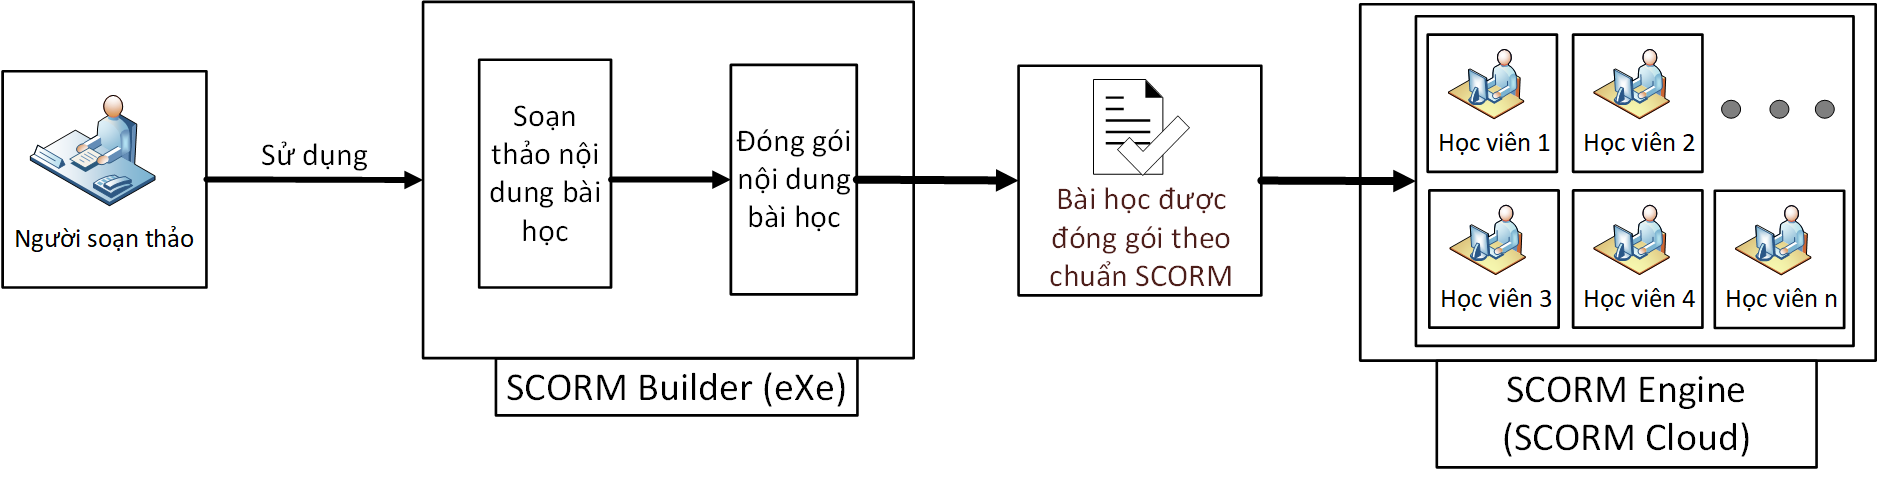
\includegraphics[width=15cm]{Chapter3/Pictures/picture34.png}
		\end{center}
		\caption{Tương tác giữa SCORM Builder và SCORM Engine}
		\label{refpicture45}
	\end{figure}
\end{center}

Hình 3.4 mô tả sự tương tác giữa SCORM Builder và SCORM Engine. Người soạn thảo sẽ sử dụng eXe(SCORM Builder) để thiết kế nội dung cho bài giảng, thêm các tiền điều kiện và hậu điều kiện vào mỗi bài học, sau đó đóng gói bài học theo chuẩn SCORM. Tiếp theo SCORM Cloud(SCORM Engine) sẽ hiển thị nội dung của bài học này và cung cấp một môi trường cho nhiều học viên tương tác với bài học.

\newpage

\subsection{Cấu trúc bài học được đóng gói theo chuẩn SCORM}

	\begin{center}
	\begin{figure}[htp]
		\begin{center}
			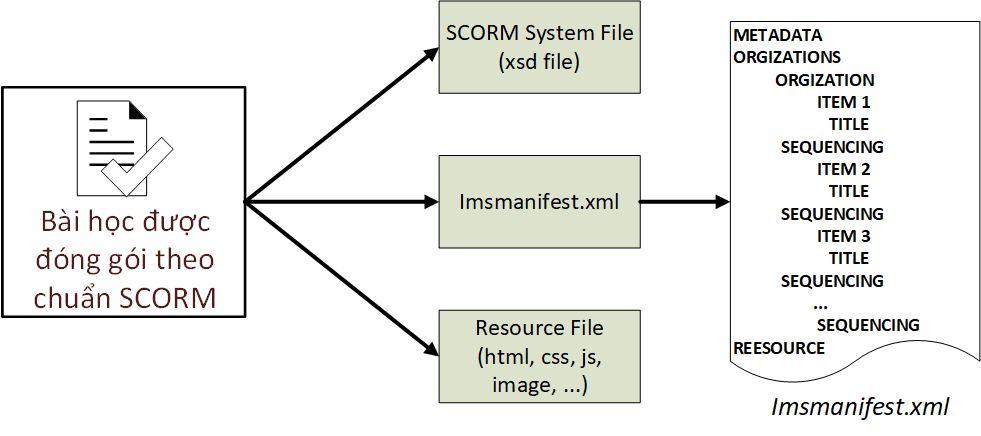
\includegraphics[width=15cm]{Chapter3/Pictures/picture35.png}
		\end{center}
		\caption{Cấu trúc bài học được đóng gói theo chuẩn SCORM}
		\label{refpicture46}
	\end{figure}
\end{center}




	Hình 3.5 liệt kê ở mức tổng quan các thành phần cần phải có trong một gói nội dung theo chuẩn SCORM. Mỗi gói nội dung sẽ bao gồm 3 thành phần chính:
	\begin{itemize}
		\item Thứ nhất là SCORM System File bao gồm những file ở định dạng xsd (XML Schema Defination) chứa những định nghĩa về các thành phần và thuộc tính trong file xml. 
		
		\item Thứ hai là file imsmanifest.xml. Định dạng XML là định dạng mô tả cấu trúc dùng để lưu trữ dữ liệu, đây là file quan trọng nhất trong gói nội dung dùng để chứa các thi6565ết lập về tổ chức nội dung bài học do người soạn thảo biên soạn. 
		
		\item Thành phần cuối cùng là các File tài nguyên sử dụng trong bài học. Các file này là các nội dung chi tiết do người soạn thảo biên soạn, thông thường sẽ là tài nguyên dạng html.
	\end{itemize}
	
	Hình 3.5 cũng cho biết vị trí thiết lập thông tin điều khiển có điều kiện cho mỗi bài học trên cây học tập. Mỗi một bài học trên cây học tập sẽ được ánh xạ tương ứng là một ITEM trong file imsmanifest.xml. Mỗi ITEM sẽ được xác định với một định danh duy nhất dùng để tham chiếu đến tài nguyên tương ứng. Trong mỗi bài học sẽ chứa một đoạn mã điều khiển có điều kiện tương ứng với các thiết lập là các ràng buộc của bài học này.\\
	 
	Sau khi có được gói nội dung được đóng gói theo chuẩn SCORM, theo quy trình như hình 3.4 thì người soạn thảo sẽ upload gói nội dung lên SCORM Cloud để mời học viên tham dự.



\subsection{Cơ chế thể hiện bài học của SCORM Engine}

	Sau khi hoàn thành việc đóng gói các nội dung và các thiết lập. Việc tiếp theo là upload gói nội dung lên SCORM Cloud và mời học viên vào tham gia bài học. Khi có một yêu cầu từ người học thì lúc này SCORM Engine sẽ đứng ra đảm nhận vai trò quản lý quá trình tham gia bài học này.\\

	SCORM Engine là một phần của Hệ Quản trị nội dung đào tạo (LMS). SCORM Engine cung cấp API cho hầu hết các ứng dụng học tập trực tuyến để đọc nội dung theo chuẩn SCORM. SCORM Engine sẽ quản lý các hoạt động như import nội dung, thực hiện khóa học và theo dõi quá trình học tập của người học. Nó là thành phần không thể thiếu đối với bất kỳ hệ thống học tập trực tuyến nào có hỗ trợ chuẩn SCORM.
	
	\begin{center}
	\begin{figure}[htp]
		\begin{center}
			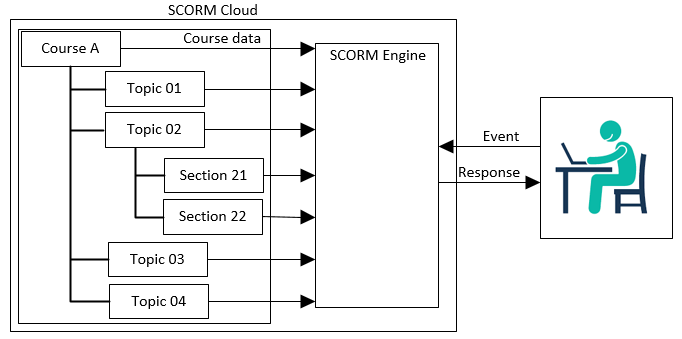
\includegraphics[width=15cm]{Chapter3/Pictures/picture36.png}
		\end{center}
		\caption{Cơ chế hoạt động của SCORM Engine (SCORM Cloud)}
		\label{refpicture47}
	\end{figure}
\end{center}


	
	Khi bắt đầu quá trình học, SCORM Engine sẽ quét tất cả các thành phần của bài học. Các thành phần của bài học này được lưu trữ trên SCORM Cloud từ file imsmanifest.xml đã được upload và các thông tin này được ánh xạ thành mô hình cây bài học như hình 3.6 mô tả.\\
	
	Tiếp đến, SCORM Engine khởi tạo tất cả các thuộc tính ở tất cả các bài học trên cây học tập bao gồm các thuộc tính định danh và thuộc tính trạng thái. SCORM Engine quản lý các thông số bài học theo cơ chế Event-Driven, với mỗi hoạt động của người học thực hiện trên cây học tập thì SCORM Engine sẽ quét lại toàn bộ các thuộc tính trạng thái ở từng bài học của cây học tập và kiểm tra các điều kiện điều khiển đã được thiết lập trên mỗi bài học. Ở từng hoạt động của người học thì các thông tin điều khiển có điều kiện cũng đều được SCORM Engine kiểm tra lại.\\
	
	Mỗi bài học trên cây sẽ có một tập các thuộc tính trạng thái. Những thiết lập điều khiển có điều kiện này sẽ dựa vào tập các thuộc tính này mà đưa ra hai trạng thái là \textbf{\textit{enable}} hoặc \textbf{\textit{disable}} đối với người học. Cụ thể về tập thuộc tính trạng thái này sẽ được trình bày trong phần sau.



\subsection{Cơ chế hiện thực các luật điều khiển có điều kiện}

\subsubsection{Thuộc tính trạng thái trên mỗi bài học}

\begin{center}
	\begin{figure}[htp]
		\begin{center}
			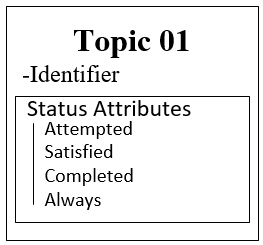
\includegraphics[width=5cm]{Chapter3/Pictures/picture37.png}
		\end{center}
		\caption{Các thuộc tính trong một bài học}
		\label{refpicture48}
	\end{figure}
\end{center}


Mỗi một bài học trên cây học tập ngoài thuộc tính định danh có giá trị duy nhất với mỗi bài học còn có một tập các thuộc tính về trạng thái đối với nhiều trường hợp khác nhau. Hình 3.7 là các thuộc tính có trong một node bao gồm các thuộc tính \textbf{Attempted}, \textbf{Satisfied}, \textbf{Completed} và \textbf{Always}. Các thuộc tính trạng thái này có miền giá trị là Boolean, được dùng để xác định trạng thái của một bài học cụ thể như sau:

\begin{table}[!htp]
	
	\begin{tabular}{|l|p{10.8cm}|}
		\hline 
		\textbf{Thuộc tính trạng thái} & \hspace{4.6cm}\textbf{Ý nghĩa}\\ 
		\hline 
		Attempted & Giá trị khởi tạo là \textbf{False}.\newline \textbf{True} nếu như node bài học này được người học xem qua.
		\\ 
		\hline 
		Satisfied & Giá trị khởi tạo là \textbf{False}.\newline \textbf{True} nếu như node bài học này được người học xem qua và nếu trong node bài học có nội dung cần phải đạt thì điều kiện sẽ \textbf{True} khi đạt các nội dung đó.
		\\ 
		\hline 
		Completed & Giá trị khởi tạo là \textbf{False}.\newline \textbf{True} nếu các nội dung trong node đều được người học xem qua mà không cần phải đạt.
		\\ 
		\hline 
		Always & Giá trị khởi tạo là \textbf{True}.\newline Thuộc tính này không thể thay đổi giá trị. Đây là một thuộc tính được chuẩn SCORM mô tả với mục đính sử dụng riêng.
		\\ 
		\hline 
	\end{tabular} 
	\caption{Các thuộc tính trạng thái của một bài học}
	\label{reftable41}
\end{table}



Nguyên tắc của việc chuyển điều khiển mà chuẩn SCORM mô tả là dựa vào sự thay đổi của các thuộc tính trạng thái này mà đưa ra các hành động tương ứng. Người học và người biên soạn không thể thiết lập giá trị cho các thuộc tính này, các giá trị này sẽ do SCORM Engine quản lý và sẽ thay đổi trong quá trình học của người học. Phần sau sẽ trình bày nguyên tắc SCORM Engine sử dụng các thuộc tính trạng thái này để chuyển trạng thái các node.\\


\subsubsection{Các luật điều khiển có điều kiện}

		\begin{center}
	\begin{figure}[htp]
		\begin{center}
			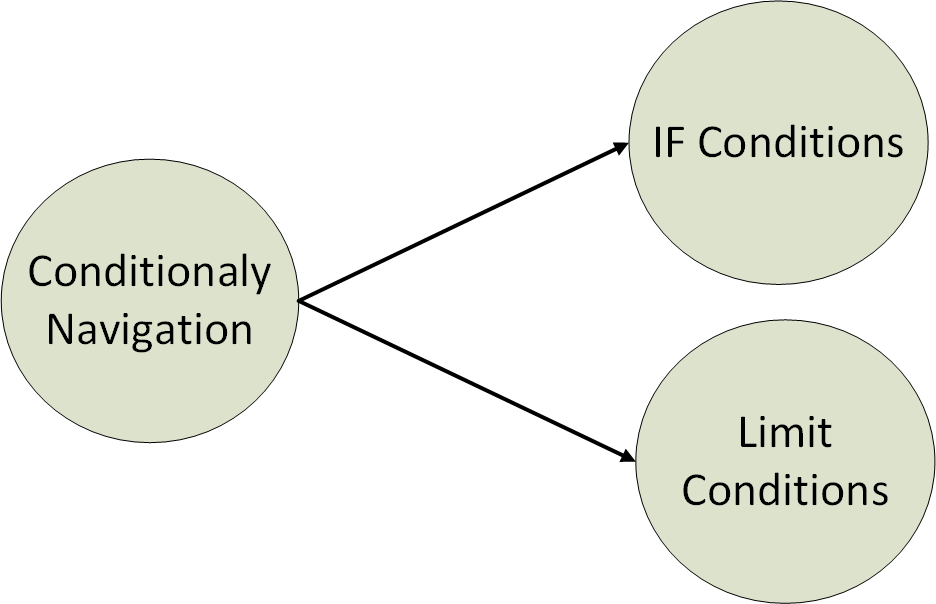
\includegraphics[width=10cm]{Chapter3/Pictures/picture38.png}
		\end{center}
		\caption{Các loại luật điều khiển có điều kiện}
		\label{refpicture49}
	\end{figure}
\end{center}

	Luật điều khiển có điều kiện (Conditionaly Navigation) là một tập hợp gồm không hoặc nhiều điều kiện có thể ảnh hưởng lên bài học trong cây học tập. Có 2 loại luật điều khiển có điều kiện có thể được áp dụng trên các bài học là IF Conditions và Limit Conditions như hình 3.8 mô tả. IF Conditons là tập những ràng buộc dựa vào các trạng thái của các bài học trên cây học tập. Limit Conditions là các ràng buộc về giới hạn, ví dụ như thời gian học trên mỗi bài học và số lần học tập tối đa trên mỗi bài học.\\

 	\textbf{a. IF Conditions}\\
	
	IF Conditions là tập hợp các luật tuân theo cấu trúc \textbf{(IF [condition\_set] THEN [action])}. Hình 3.9 là các tập hợp về những luật điều khiển và các hành động tương ứng được đưa ra. Conditions là các điều kiện được đưa ra dựa trên các thuộc tính trạng thái của các bài học trên cây học tập và các thuộc tính này đã được trình bày ở phần đầu của chương. Rule Actions bao gồm các hành động tương ứng cho các Tiền điều kiện (PreCondition) và Hậu điều kiện (PostCondition). Các thông tin về IF Conditions được đặt trong cặp thẻ <imsss:SequencingRules> trong file imsmanifest.xml theo cấu trúc bài học được đóng gói theo chuẩn SCORM ở hình 3.5.
	
	
		\begin{center}
		\begin{figure}[htp]
			\begin{center}
				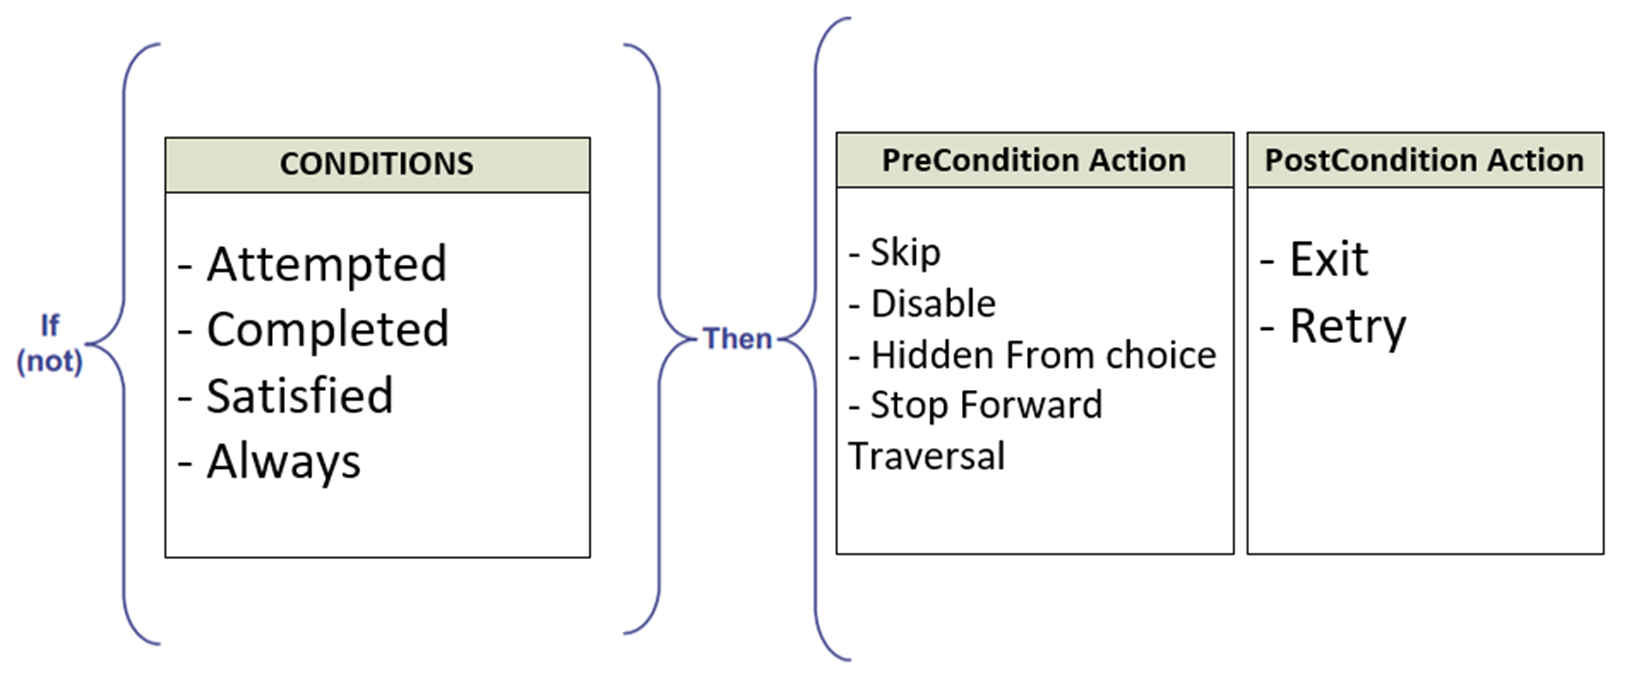
\includegraphics[width=15cm]{Chapter3/Pictures/picture39.png}
			\end{center}
			\caption{Những luật điều khiển và các hành động tương ứng}
			\label{refpicture410}
		\end{figure}
	\end{center}

	Phía sau Then là tập hợp các hành động được SCORM Engine chịu trách nhiệm xử lý khi thỏa mãn điều kiện đưa ra. If Conditions chia các hành động ra thành hai hướng xử lý là hành động cho điều kiện vào và hành động cho điều kiện ra.\\
	
	\begin{itemize}
		\item \textbf{Xử lý cho điều kiện vào}: Tập các hành động đưa ra cho bài học hiện tại để xác định khi nào người học có thể đi vào được bài học này. Ví dụ A có 2 bài học con là B và C, ta thiết lập điều kiện vào trên C là B \textbf{not satisfied} và hành động đưa ra là \textbf{\textit{disable}}. Khi đó, C sẽ bị SCORM Engine \textbf{\textit{disable}} đi cho đến khi các hoạt động trong B \textbf{satisfied} thì C sẽ \textbf{\textit{enable}} và người học có thể lựa chọn.
		
		\item \textbf{Xử lý cho điều kiện ra}: Tập các hành động đưa ra khi đi ra khỏi bài học hiện tại. Ví dụ A có 2 bài học con là B và C, ta thiết lập điều kiện ra ở B là B \textbf{not completed} và hành động đưa ra là \textbf{retry}. Khi đó nếu người học vào B và các hành động trong B chưa được người học xem qua hết thì khi ra khỏi B SCORM Engine sẽ thực hiện lệnh \textbf{retry} và người học sẽ xem lại nội dung B cho đến khi hoàn tất.
	\end{itemize}

	\vspace{1cm}
	
	Có thể kết hợp nhiều Conditons với nhau bằng các toán tử AND hoặc OR. Các toán tử này được thiết lập bằng cách khai báo thêm một thuộc tính \textbf{conditionCombination} khi khai báo cặp thẻ \textbf{<imsss:SequencingRules>. conditionCombination=“any”} cho toán tử OR hoặc \textbf{conditionCombination=“all”} cho toán tử AND.\\
	
	Với mỗi trường hợp ta sẽ có tập hợp những hành động đưa ra tương ứng. Các hành động này được liệt kê như trong bảng 3.2.
	
	\newpage
	
\begin{table}[!htp]
	
	\begin{tabular}{|p{4cm}|p{10.8cm}|}
		\hline 
		\textbf{Trường hợp} & \hspace{4.6cm}\textbf{Hành động} 
		\\
		\hline 
		Xử lý điều kiện vào của bài học hiện tại. & 
		\textbf{\textit{Skip}} – bài học hoạt động này sẽ không được tham gia vào trình duyệt cây.\newline
		\textbf{\textit{Disabled}} – Hoạt động này sẽ bị vô hiệu hóa và không thể tham gia vào quá trình duyệt cây.\newline
		\textbf{\textit{Hidden from Choice}} – Hoạt động này sẽ không thể bị target và bị ẩn khỏi cây.\newline
		\textbf{\textit{Stop Forward Traversal}} – Không cho phép duyệt các phần tử con của bài học Activity này.
		\\
		\hline 
		Xử lý điều kiện ra khi thoát khỏi bài học hiện tại. & 
		\textbf{\textit{Exit}} – Action thoát khỏi nội dung này bình thường.\newline
		\textbf{\textit{Retry}} – Action đưa yêu cầu làm lại nội dung này.
		\\
		\hline 
	\end{tabular} 
	\caption{Các điều kiện và hành động tương ứng của một bài học}
	\label{reftable42}
\end{table}	
	

 \textbf{b. Limit Conditions}\\
	
	Limit Conditions đưa ra các ràng buộc về giới hạn cho bài học hiện tại trên cây học tập. Limit Conditions chỉ ra các thông số giới hạn mà người học có thể thực hiện được như số lần làm bài tối đa, thời gian học tối thiểu trong một nội dung. Được đặt trong cặp thẻ <LimitConditions> trong file imsmanifest.xml.\\
	
	Chuẩn SCORM quy định có 2 ràng buộc về điều kiện giới hạn như sau:
	
	\begin{itemize}
		\item \textbf{Attempt Limits}: Ràng buộc về số lần học tối đa đối với một nội dung. Được hiện thực bằng 2 tham số: 
			\begin{itemize}
				\item \textbf{Limit Condition Attempt Control:} có giá trị Boolean để quy định rằng nội dung này có bị ảnh hưởng bởi ràng buộc Limit Condition này hay không. 
				
				\item \textbf{Limit Condition Attempt Limit:} có giá trị là Non-negative Interger quy định số lần học tối đa đối với một nội dung. Ví dụ nếu tham số này có giá trị 3 thì người học có thể xem nội dung này 3 lần trong quá trình học.
				
			\end{itemize}
			
		\item \textbf{Attempt Absolute Durations:} Ràng buộc về thời gian học tối thiểu đối với một nội dung trong cây học tập. Được hiện thực bằng 2 tham số: 
			\begin{itemize}
	
				\item \textbf{Limit Condition Attempt Absolute Duration Control:} có giá trị Boolean để quy định rằng nội dung này có bị ảnh hưởng bởi ràng buộc Limit Condition này hay không. 
				
				\item \textbf{Limit Condition Attempt Absolute Duration Limit:} có giá trị là Duration với Acurarcy 0.1 second quy định thời gian tối thiểu đối với một nội dung. Nếu thiết lập giá trị là 60s thì người học phải xem nội dung này tối thiểu trong một phút mới có thể chuyển sang nội dung tiếp theo.

			\end{itemize}
		
	\end{itemize}
	
	\newpage
	

\section{Hiện thực chức năng}


		\begin{center}
	\begin{figure}[htp]
		\begin{center}
			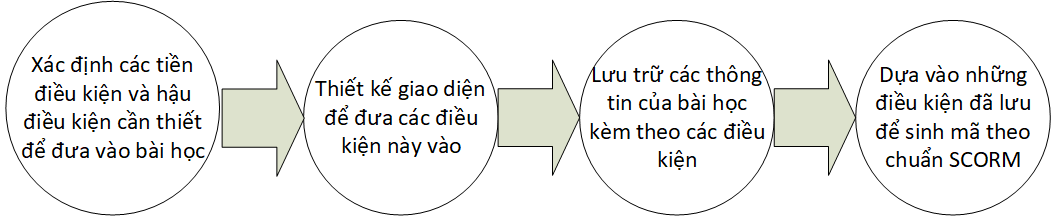
\includegraphics[width=15cm]{Chapter3/Pictures/picture310.png}
		\end{center}
		\caption{Quy trình hiện thực chức năng điều khiển có điều kiện}
		\label{refpicture413}
	\end{figure}
\end{center}


	Hình 3.10 là quy trình hiện thực chức năng do nhóm đề xuất thực hiện. Bao gồm bốn bước chính. Bước một là xác định các tiền điều kiện và hậu điều kiện cần thiết để đưa vào bài học. Ở bước hai sẽ thiết kế giao diện dành cho người soạn thảo có thể đưa các điều kiện này vào trong bài học. Bước ba là xử lý việc lưu trữ thông tin của bài học đã được thêm các điều kiện vào. Bước cuối cùng sẽ dựa vào những điều kiện đã lưu để sinh mã có chức năng điều khiển có điều kiện cho từng bài.\\
	
	
	
\subsection{Xác định các tiền điều kiện và hậu điều kiện}

	Sau khi tìm hiểu các ràng buộc về điều khiển có điều kiện có trong đặc tả chuẩn SCORM 2004. Nhóm đưa ra các ràng được sẽ được hiện thực trong chức năng. Tiền điều kiện là các ràng buộc cần để có thể vào được nội dung này. Hậu điều kiện là các ràng buộc để ra khỏi nội dung này.


\begin{itemize}
	\item \textbf{PreCondition (Tiền điều kiện):} Ràng buộc về nội dung trước cần thõa mãn. Ví dụ A có 2 bài học con là B và C, ta set PreCondition trên C là B \textbf{\textit{satisfied}}. Khi đó  các hoạt động trong B nếu \textbf{NOT} \textbf{\textit{satisfied}} thì action là C \textbf{\textit{disable}}.
	
	\item \textbf{PostConditon (Hậu điều kiện):}
	\begin{itemize}
		\item Ràng buộc về thời gian học trong một bài học. Nếu trong bài học có thiết lập thời gian học, người học sẽ không thể ra khỏi nội dung này nếu chưa hết thời gian quy định.
		
		\item Nếu trong bài học có SCORM Quiz thì đưa ra những lựa chọn ràng buộc về SCORM Quiz, bao gồm các tùy chỉnh: Đạt một hoặc nhiều SCORM Quiz, các SCORM Quiz cần đạt này do người biên soạn quy định hoặc đạt một trong số các SCORM Quiz có trong bài học.
	\end{itemize}

	
\end{itemize}

	Sau khi xác định được các ràng buộc sẽ thể hiện trong chức năng, phần tiếp theo sẽ trình bày quá trình hiện thực chức năng bao gồm 3 bước còn lại trong quy trình đưa ra ở hình 3.10.


\subsection{Thiết kế giao diện để đưa các điều kiện vào trong bài học}

	Giao diện Sequencing Config sẽ là duy nhất  đối với từng bài học. Với những bài học có SCORM Quiz sẽ có thêm các thiết lập về SCORM Quiz, những bài học không có SCORM Quiz sẽ không xuất hiện những tùy chọn này.\\
	
	Giao diện Sequencing Config sẽ có hai Tag Panel chính là PreCondition và PostCondition. PreCondition chứa thiết lập về tiền điều kiện và PostCondition chứa thiết lập về hậu điều kiện cho bài học.\\
	
	Hình 3.11 là giao diện thiết lập tiền điều kiện, giao diện này sẽ có một combo box yêu cầu chọn nội dung trước cần thỏa mãn, người học cần thỏa mãn nội dung được chọn mới được vào học bài này.

		\begin{center}
	\begin{figure}[htp]
		\begin{center}
			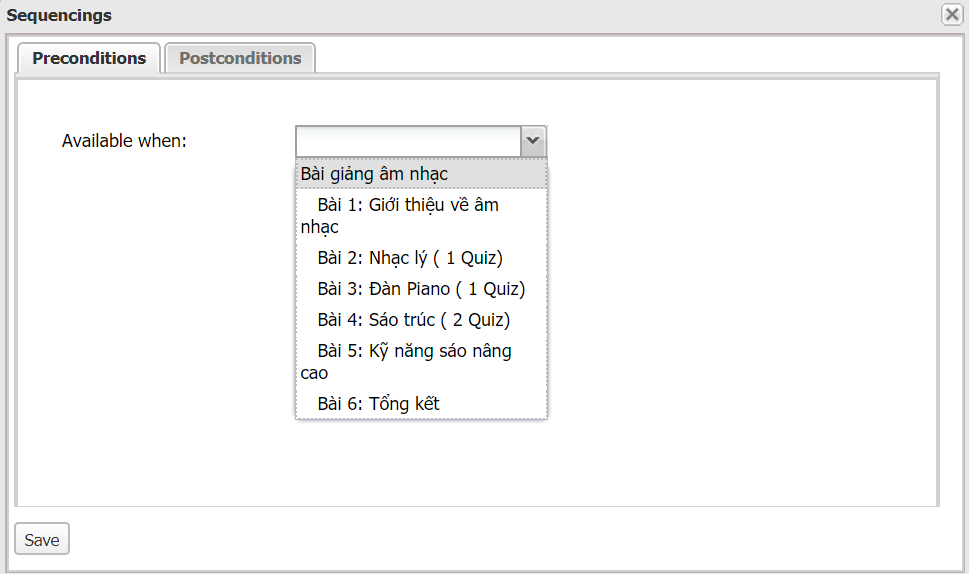
\includegraphics[width=15cm]{Chapter3/Pictures/picture311.png}
		\end{center}
		\caption{Giao diện thiết lập tiền điều kiện}
		\label{refpicture413}
	\end{figure}
\end{center}

	Khi giao diện thiết lập tiền điều kiện này xuất hiện, trình duyệt sẽ gửi yêu cầu rằng người soạn thảo đang cần thực hiện các thiết lập điều khiển có điều kiện, lúc này máy chủ thông qua việc sử dụng kỹ thuật Ajax để lấy dữ liệu. Máy chủ sẽ phân tích yêu cầu này và gửi danh sách các bài học có trong khóa học lưu dưới dạng JSON cho trình duyệt. Trình duyệt sẽ phân tích nội dung nhận được này và thể hiện thành các mục trong combobox.


		\begin{center}
	\begin{figure}[htp]
		\begin{center}
			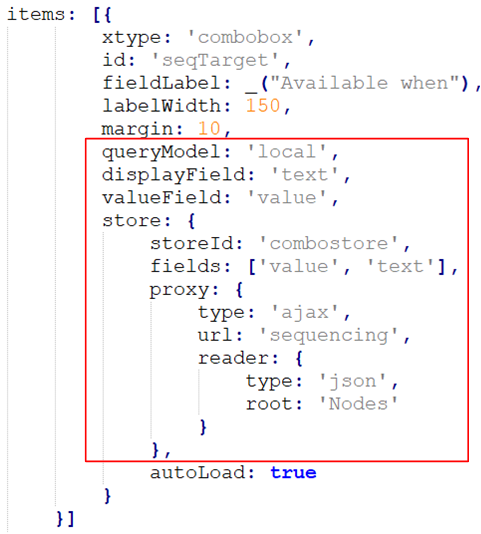
\includegraphics[width=7cm]{Chapter3/Pictures/picture312.png}
		\end{center}
		\caption{Kỹ thuật Ajax để lấy dữ liệu trong combobox}
		\label{refpicture413}
	\end{figure}
\end{center}


	Hình 3.12 là đoạn mã hiện thực combobox trong giao diện thiết lập tiền điều kiện sử dụng khung thức của ExtJS để hiện thực. Ở đây, dữ liệu JSON lấy từ url:sequencing sẽ được lưu trữ thành một data store có ID là "combostore" gồm 2 trường “value” và “text”. Combobox sẽ lấy trường hiển thị (display Fiels) là trường “text” và trường giá trị(valueField) là “value”. Hình 3.13 là cú pháp combobox đối chiếu với Javascript thuần túy.

		\begin{center}
	\begin{figure}[htp]
		\begin{center}
			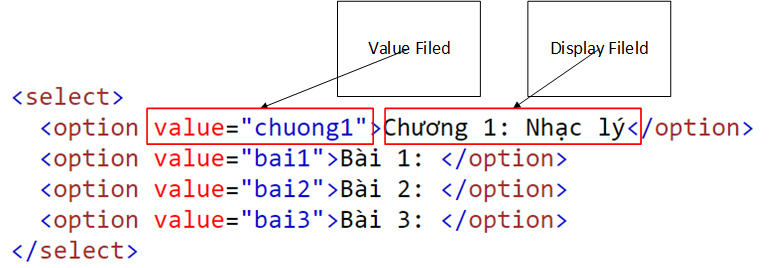
\includegraphics[width=15cm]{Chapter3/Pictures/picture313.png}
		\end{center}
		\caption{Combobox theo Javascript thuần túy}
		\label{refpicture413}
	\end{figure}
\end{center}


		\begin{center}
	\begin{figure}[htp]
		\begin{center}
			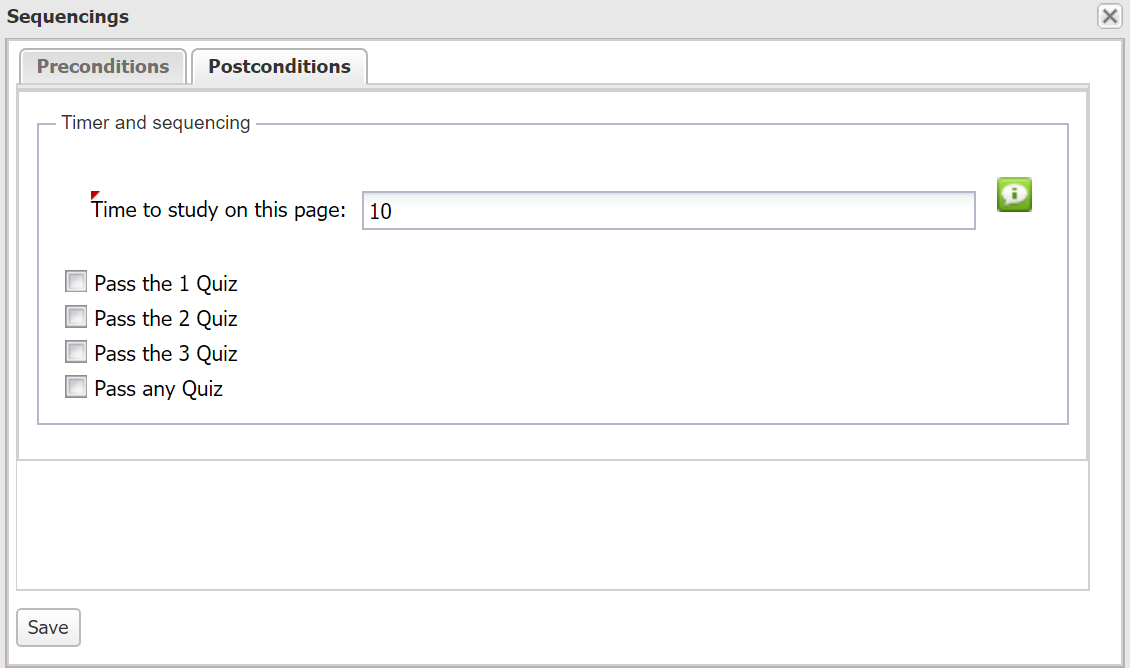
\includegraphics[width=15cm]{Chapter3/Pictures/picture314.png}
		\end{center}
		\caption{Giao diện thiết lập hậu điều kiện}
		\label{refpicture415}
	\end{figure}
\end{center}


Hình 3.14 là giao diện thiết lập các hậu điều kiện. Giao diện này sẽ có một textField yêu cầu người soạn thảo nhập vào thời gian tối thiểu mà người học sẽ phải xem nội dung này, đơn vị của thời gian sẽ tính bằng giây.
Nếu như trong nội dung bài học này mà người soạn thảo có thiết lập SCORM Quiz thì các thiết lập về SCORM Quiz sẽ xuất hiện ở đây bao gồm các checkbox yêu cầu cần đạt đối với từng SCORM Quiz và có thêm checkbox “Pass any Quiz” cho điều kiện chỉ cần đạt một trong bất kỳ SCORM Quiz nào là nội dung này sẽ được thõa mãn. Sau khi lấy các thông số người dùng nhập vào, sử dụng các phương thức gửi và nhận dữ liệu do Nevow cung cấp để gửi và lưu trữ thông tin ở phía máy chủ.


\subsection{Lưu thông tin bài học do người soạn thảo thiết lập}

Như đã trình bày ở phần kiến trúc hệ thống công cụ eXe Learning. Hệ thống hoạt động theo mô hình Client-Server và các phương thức xử lý đều được thực hiện ở phía Server. Sau khi người soạn thảo thiết lập các điều kiện điều khiển trình tự ở bước trên, thì dữ liệu này sẽ phải được gửi về phía server để tiến hành bước tiếp theo.

		\begin{center}
	\begin{figure}[htp]
		\begin{center}
			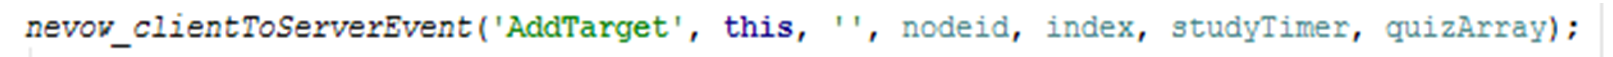
\includegraphics[width=15cm]{Chapter3/Pictures/picture315.png}
		\end{center}
		\caption{Phương thức Nevow gửi dữ liệu về Server}
		\label{refpicture416}
	\end{figure}
\end{center}

	Hình 3.15 là phương thức gửi dữ liệu về phía máy chủ được Nevow cung cấp, Các thuộc tính lần lượt là nodeid, index, studyTimer, quizList với nodeid là IdTarget lưu trữ bài học mục tiêu cần thỏa mãn của bài học hiện tại, index là vị trí của bài học hiện tại trên cây bài học, studyTimer lưu trữ thời gian học tối đa trong bài học hiện tại và quizList lưu trữ danh sách các Quiz cần Pass của bài học hiện tại nếu có.\\

	
	Như vậy, cần thay đổi các thiết kế ban đầu về một số cấu trúc lưu trữ dữ liệu ở phía server để có thể lưu trữ được các nội dung này. Như đã trình bày eXe Learning quản lý nội dung của các bài học theo mô hình cây. Mỗi bài học trong khóa học sẽ được lưu trữ là một bài học trong cây học tập. Mỗi bài học sẽ được thêm ba thuộc tính tương ứng với ba điều kiện điều khiển có điều kiện.


		\begin{center}
	\begin{figure}[htp]
		\begin{center}
			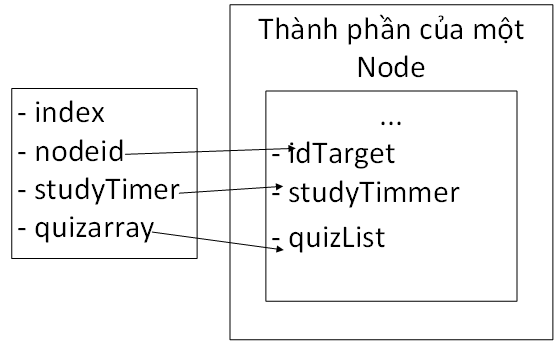
\includegraphics[width=15cm]{Chapter3/Pictures/picture316.png}
		\end{center}
		\caption{Lưu trữ các thiết lập trên bài học}
		\label{refpicture413}
	\end{figure}
\end{center}

Hàm xử lý nhận các tham số mà hình 3.15 cung cấp sẽ được hiện thực như hình 3.16 mô tả. Đầu tiên sẽ dựa vào tham số index nhận được, tìm ra bài học cần thiết lập. Sau khi tìm vị trí bài học hiện tại được lưu trữ trên máy chủ thông qua tham số index nhận được, máy chủ sẽ lưu trữ các tham số tiếp theo trong bài học vừa tìm được. idTarget là thuộc tính cho bài học mục tiêu cần thõa mãn. studyTimer là thuộc tính cho thời gian học tối thiểu. quizList là danh sách các quiz cần phải đạt để nội dung này thỏa mãn.



\subsection{Sinh mã điều khiển có điều kiện theo chuẩn SCORM}

	Như đã trình bày ở phần đầu chương, các đoạn mã điều khiển có điều kiện được tạo ra trong file imsmanifest.xml. Phương thức sinh ra chuỗi để ghi vào file này được hiện thực trong module Export. \\
	
	File scormexport.py khai báo hai lớp chính là Manifest và ScormExport. Lớp Manifest chứa các phương thức sinh mã ra file imsmanifest.xml. Lớp ScormExport chứa các phương thức gộp các file thành phần lại với nhau và đóng gói thành file có định dạng zip. Mã điều khiển có điều kiện được sinh ra trong file imsmanifest.xml, do đó nhóm sẽ hiện thực thêm một phương thức để sinh ra các đoạn mã này trong class Manifest. Quá trình sinh ra các đoạn mã này như sau:

	
	\begin{center}
	\begin{figure}[htp]
		\begin{center}
			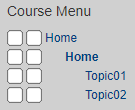
\includegraphics[width=4cm]{Chapter3/Pictures/picture317.png}
		\end{center}
		\caption{Course Menu trong ví dụ}
		\label{refpicture411}
	\end{figure}
\end{center}


Đây là một ví dụ tổng hợp về các luật điều khiển có điều kiện mà chuẩn SCORM mô tả đã trình bày ở các phần trên. Hình 3.17 là mô hình cây học tập được đưa ra trong ví dụ gồm 1 nội dung với 2 topic là \textbf{Topic01} và \textbf{Topic02}.


\begin{center}
	\begin{figure}[htp]
		\begin{center}
			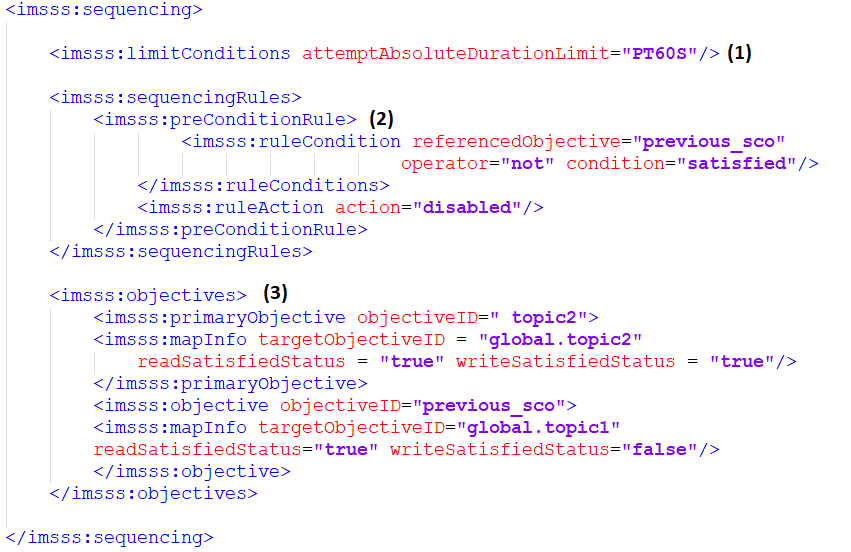
\includegraphics[width=15cm]{Chapter3/Pictures/picture318.png}
		\end{center}
		\caption{Đoạn mã chứa thông tin điều khiển có điều kiện trong file imsmanifest.xml}
		\label{refpicture412}
	\end{figure}
\end{center}

\newpage

Hình 3.18 là những đặc tả về thông tin điều khiển có điều kiện theo chuẩn SCORM được trình bày sang file imsmanifest.xml. XML là ngôn ngữ cấu trúc dùng để chứa dữ liệu và liệt kê các thành phần dữ liệu, do đó cấu trúc IF [conditions\_set] THEN [Action] sẽ không có hình thái rõ ràng như các ngôn ngữ khác. File imsmanifest.xml này sẽ chỉ lưu dữ liệu của cấu trúc trên và việc thực thi sẽ do SCORM Engine thực hiện.\\

Đoạn mã trong hình 3.18 được đặt trong <item> có định danh là \textbf{\textit{topic2}}, tương ứng với \textbf{Topic02} trên cây học tập ở hình 3.17. Đoạn mã trên có 3 phần riêng biệt với các nhiệm vụ khác nhau. \\

Phần \textbf{(3)} là phần khai báo các đối tượng sử dụng bao gồm một primary Object và một Object. Khai báo Primary Object là khai báo định danh cho chính Item hiện tại, ở đây là \textbf{\textit{topic2}}. Khi thực thi, trên bài học này cho phép SCORM Engine có thể đọc và ghi thuộc tính \textbf{\textit{satisfied}}. Khai báo Objective là khai báo các đối tượng tham chiếu đến, ở đây khai báo có tên là \textbf{\textit{previous\_sco}} dùng để tham chiếu đến bài học nội dung có định danh là \textbf{\textit{topic1}}. Khi thực thi trên bài học này chỉ có thể đọc thuộc tính \textbf{\textit{satisfied}} của Object Topic01 nhưng không thể ghi thuộc tính \textbf{\textit{satisfied}} của \textbf{Topic01}.\\

Phần \textbf{(2)} là triển khai các điều kiện vào với điều kiện đưa ra là \textbf{\textit{previous\_sco}} \textbf{NOT} \textbf{satisfied} và hành động đưa ra là \textbf{\textit{disable}}. Khi định danh mà \textbf{\textit{previous\_sco}} tham chiếu đến là \textbf{\textit{topic1}} chưa thỏa mãn thì \textbf{\textit{topic2}} sẽ bị \textbf{disable}. Khi nào các thành phần trong \textbf{\textit{topic1}} đã thỏa mãn yêu cầu thì \textbf{\textit{topic2}} sẽ được đưa vào lựa chọn.\\

Phần \textbf{(1)} là triển khai Limit Conditions với điều kiện đưa ra là Limit Condition Attempt Absolute Duration Limit = 60 second. Điều kiện này quy định thời gian học đối với topic 2 này là 60s.



\subsection{Kết quả thực hiện}

Sau khi đóng gói nội dung khóa học có các thông tin điều khiển có điều kiện bằng công cụ eXe. Nhóm tiến hành upload lên SCORM Cloud để xem kết quả và so sánh với gói nội dung không có thông tin điều khiển có điều kiện.	
	
			\begin{center}
		\begin{figure}[htp]
			\begin{center}
				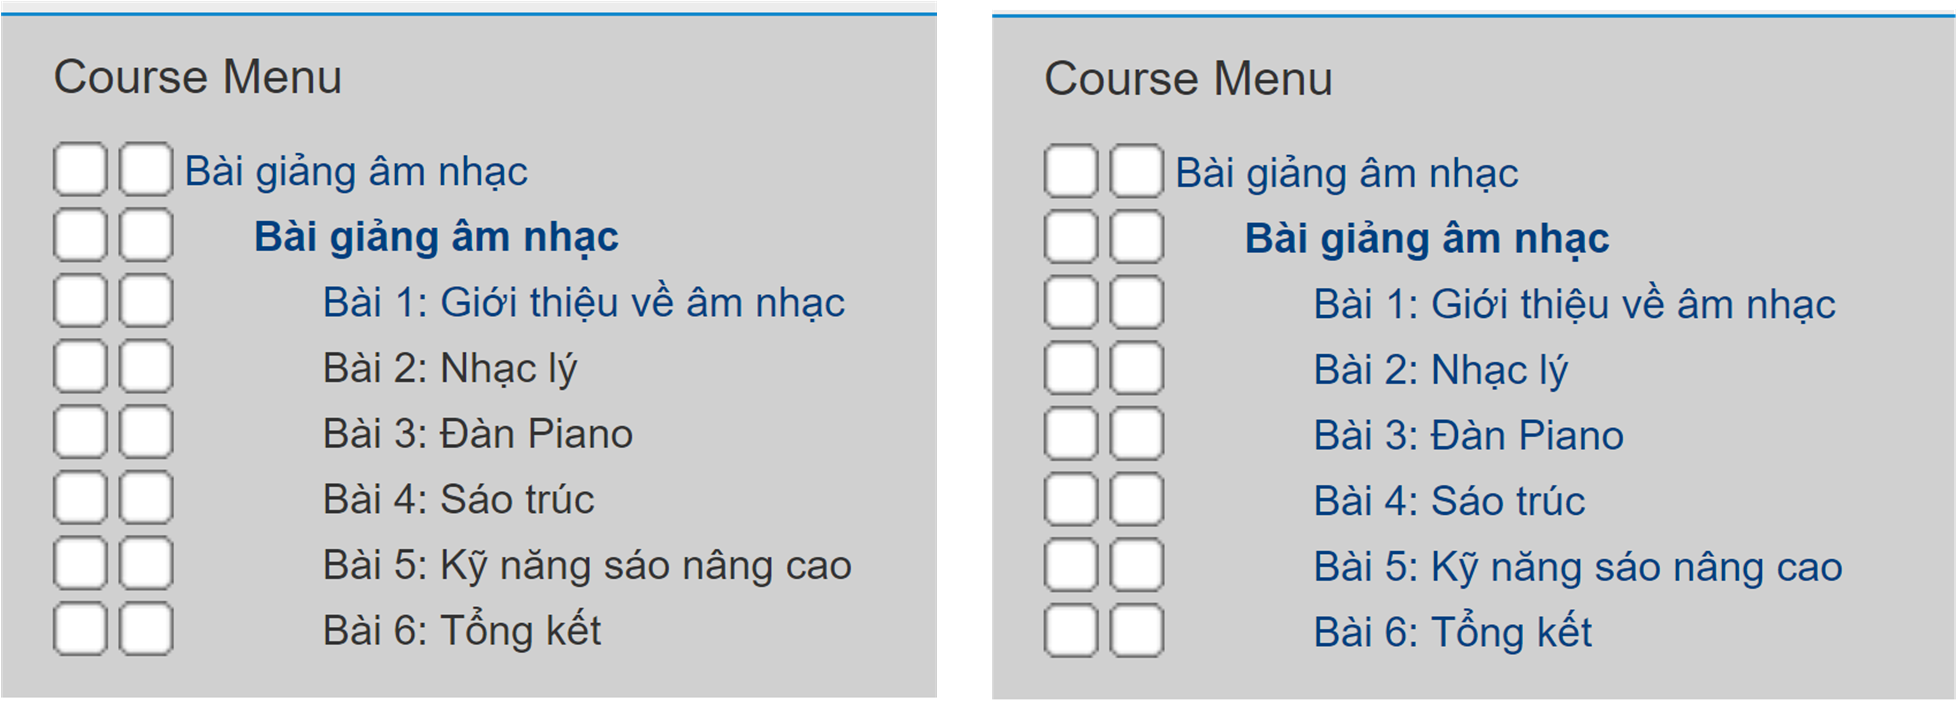
\includegraphics[width=15cm]{Chapter3/Pictures/picture319.png}
			\end{center}
			\caption{Giao diện của hai khóa học trên SCORM Cloud}
			\label{refpicture417}
		\end{figure}
	\end{center}
	
	Hình 3.19a là khóa học không có thông tin điều khiển có điều kiện và hình 3.19b là khóa học đã thiết lập thông tin điều khiển có điều kiện. Rõ ràng ta thấy hình 3.19b yêu cầu người học phải tuân theo một lộ trình do người biên soạn thiết lập sẵn. Trong mỗi bài học sẽ có những yêu cầu riêng như học trong một khoản thời gian nhất định hoặc pass các bài quiz có trong bài học hoạt động. Còn hình 3.19a thì người học có thể tham gia vào bất kì hoạt động nào có trên cây.

\subsection{Hạn chế của chức năng}	

	Chưa đi sâu vào nghiên cứu ý kiến và nhu cầu của người biên soạn. Nhu cầu của người biên soạn đóng vai trò quan trọng trong việc thiết kế chức năng của ứng dụng. Do cộng đồng người sử dụng eXe Learning tương tác với nhau khá chậm nên nhóm gặp rất nhiều khó khăn trong việc tiến hành thu thập thông tin về nhu cầu của người sử dụng. \\
	
	Nhóm chỉ tập trung vào nghiên cứu và thực hiện một số ràng buộc tương đối đơn giản.  Chưa khai thác được hết toàn bộ sức mạnh của các mã SCORM được đặc tả trong chuẩn SCORM, không sử dụng được hết tất cả các Rule Conditions (Luật điều kiện) là một trong những hạn chế lớn của chức năng.








